\documentclass[dvipdfmx]{jarticle}
\usepackage{url}
\usepackage{graphicx}
\title{情報技術者と社会第5回レポート}
\author{ソフトウェア科学コース\\09B22084山久保孝亮}
\date{\today}

\begin{document}
\maketitle
\section{課題1}
今回のhtmlファイルの実行結果は以下の図1のようになった.
\begin{figure}[h]
    \centering
    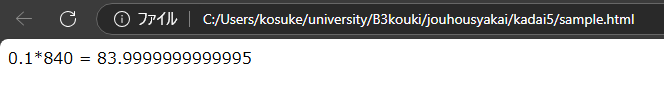
\includegraphics[width=12cm]{kadai5-1.png}
    \caption{htmlファイルの実行結果}
\end{figure}
\\今回使用した環境は,OSはWindows11でブラウザはMicrosoft Edgeである.
\section{課題2}
今回の授業の穴埋めは以下の表のようになる.
\begin{table}[h]
    \centering
    \begin{tabular}{|c|c|}
        \hline
        ページ番号 & 穴埋めの内容\\\hline\hline
        4 & 同姓同名の人と間違えられた\\\hline
        5 & independent verification,alidation\\\hline
        6 & fly\\\hline
        8 & オーバーフロー\\\hline
        17 & 自動運転\\\hline
    \end{tabular}
    \caption{穴埋めの内容}
\end{table}
\end{document}